\section{Preliminaries}
\label{section:preliminaries}

In this section, we will focus on the vocabulary used in this report, along with the first known results required for the next sections. Let's start with some notation that will be used throughout this report. For an integer $k$, by $[k]$ we denote $\{1, \dots, k\}$. For a graph $G$, by $V(G)$ we denote the vertices of $G$ and by $E(G)$ we denote the edges of $G$. If $X \subseteq V(G)$, then $G - X$ denotes the graph $G'$ obtained by removing every vertex in $X$ and every edge with an endpoint in $X$. Unless stated otherwise, $n$ always refers to $|V(G)|$, while $m$ refers to $|E(G)|$. 
% For a set $X$, by $X = X_1 \uplus \dots \uplus X_m$ we denote a disjoint partition of $X$.
%  (i.e. $X_1 \cup \dots \cup X_m = X$ and $X_i \cap X_j = \emptyset$ for every $1 \leq i < j \leq m$).

\medskip

Here is a list of all \NP-hard problems we will discuss in this report:

\begin{problem}
    \problemtitle{VertexCover}
    \probleminput{A graph $G = (V, E)$, an integer $k$}
    \problemquestion{Does there exist a subset of vertices $X\subseteq V$ such that $|X| \leq k$ and $X$ is a \textit{vertex cover} of $G$, meaning every edge in $E$ has at least one endpoint in $X$?}
\end{problem}

\begin{problem}
    \problemtitle{IndependentSet}
    \probleminput{A graph $G = (V, E)$, an integer $k$}
    \problemquestion{Does there exist a subset of vertices $X \subseteq V$ such that $|X| \geq k$ and $X$ is an \textit{independent set} of $G$, meaning no two vertices in $X$ are adjacent?}
\end{problem}

\begin{problem}
    \problemtitle{$q$-Coloring}
    \probleminput{A graph $G = (V, E)$}
    \problemquestion{Can the vertices of $G$ be colored with $q$ colors such that no two adjacent vertices share the same color. In other words, does there exist a function $f : V \mapsto [q]$ where $f(u) \neq f(v)$ for every edge $\{u,v\} \in E$?}
\end{problem}

% \begin{problem}
%     \problemtitle{MaxCut}
%     \probleminput{A graph $G = (V, E)$, an integer $k$}
%     \problemquestion{Can the vertex set $V$ be partitioned into two disjoint subsets, $V = V_1 \uplus V_2$, such that the number of edges between $V_1$ and $V_2$ is at least $k$?}
% \end{problem}

% \begin{problem}
%     \problemtitle{OddCycleTransversal}
%     \probleminput{A graph $G = (V, E)$, an integer $k$}
%     \problemquestion{Does there exist a subset of vertices $X \subseteq V$ such that $|X| \leq k$ and $G - X$ is bipartite?}
% \end{problem}

\begin{problem}
    \problemtitle{DominatingSet}
    \probleminput{A graph $G = (V, E)$, an integer $k$}
    \problemquestion{Does there exist a subset of vertices $D \subseteq V$ such that $|D| \leq k$ and $D$ is a \textit{dominating set} of $G$, meaning every vertex in $V$ is either in $D$ or adjacent to a vertex in $D$?}
\end{problem}

\subsection{Treewidth}

In the introduction Section, we characterized the treewidth of a graph $G$ as a measure of its "tree-like" structure. Let's now formally define it. This parameter, initially introduced by N. Robertson and P. D. Seymour in their seminal work on graph minors \cite{robertson1986graph}, is formally defined using the concept of a \textit{tree decomposition}.

\begin{definition}[tree decomposition]
    A tree decomposition of a graph $G$ is a pair $(T, \{X_i\}_{i \in V(T)})$ where $T$ is a tree and $\{X_i\}_{i \in V(T)}$ is a collection of subsets of $V(G)$ (called \emph{bags}) such that:
    \begin{enumerate}
        \item For every vertex $v \in V(G)$, there exists at least one bag $X_i$ such that $v \in X_i$.
        \item For every edge $\{u, v\} \in E(G)$ , there exists at least one bag $X_i$ such that $\{u, v\} \subseteq X_i$.
        \item For every vertex $v \in V$, the set of bags $\{X_i\ |\ v \in X_i\}$ forms a connected subtree of $T$.
    \end{enumerate}
\end{definition}

\begin{definition}[width of a tree decomposition]
    The width of a tree decomposition $(T,\{X_i\}_{i \in V(T)})$ is the size of the biggest bag of the decomposition minus 1. Formally, it is defined as $\max_{i \in V(T)} |X_i| - 1$.
\end{definition}

\begin{definition}[treewidth]
    The treewidth of a graph $G$, denoted $\tw(G)$, is the minimum width over all possible tree decompositions of $G$. Formally, $\tw(G) = \min_{(T, \{X_i\})}\max_{i \in V(T)} |X_i| - 1$. In other words, the treewidth of $G$ is the smallest integer $k$ such that $G$ has a tree decomposition where each bag contains at most $k+1$ vertices.
\end{definition}

Although the formal definition may not immediately convey the intuition behind this measure, we provide examples (see \reffigure{fig:treewidth-example}) to help illustrate how treewidth captures the tree-like structure of a graph.

\begin{figure}
    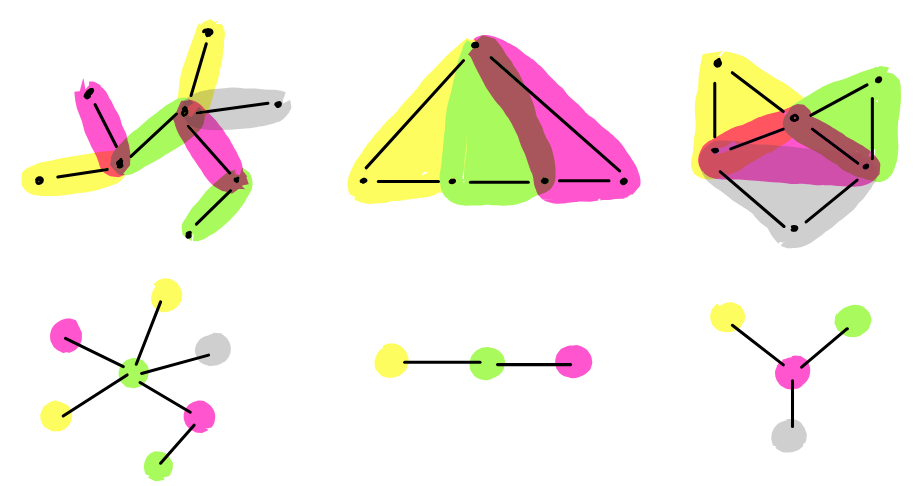
\includegraphics[width=\textwidth]{figures/treewidth-example.png}
    \caption{Examples of treewidth. (a) A tree has treewidth 1. (b) A cycle has treewidth 2. (c) A graph with treewidth 2. For each example, the bags of a tree decomposition of the graph is shown at the top, and the tree of the corresponding tree decomposition is depicted at the bottom.}
    \label{fig:treewidth-example}
\end{figure} 

\subsection{A hierarchy of parameters}

To establish a hierarchy of parameters, we first define how parameters can be compared. Formally, a parameter is a function $\pi$ that takes a graph as input and returns a number. We say that parameter $\pi_1 \lp \pi_2$ if there exists a constant $c$ such that for every graph $G$, $\pi_1(G) \leq \pi_2(G) + c$.

We will now define various parameters discussthated in this report , with an overview provided \reffigure{fig:hierarchy} illustrating how these parameters compare to each other. A portion of this hierarchy is derived from \cite{fellows2013towards}. We encourage interested readers to consult this paper for further exploration of additional parameters and their relationships.

Each time we define a parameter, we will explain its comparability with others.

\begin{tikzpicture}
    \tikzstyle{vertex} = [draw=black,fill=black,circle,inner sep=0pt,minimum size=3pt];
    \tikzstyle{possible} = [fill=green,circle,inner sep=0pt,minimum size=10pt];
    \tikzstyle{impossible} = [fill=red,circle,inner sep=0pt,minimum size=10pt];
    \tikzstyle{new} = [fill=lime,circle,inner sep=0pt,minimum size=10pt];
    \tikzstyle{result} = [draw=black,circle,dashed,thick,inner sep=0pt,minimum size=20pt];
    \tikzstyle{edge} = [draw=black,thick];
    \tikzstyle{possibleedge} = [draw=green,line width=5pt];
    \tikzstyle{impossibleedge} = [draw=red,line width=5pt];
    \tikzstyle{newedge} = [draw=lime,line width=5pt];

    % This is an invisible rectangle which draw the picture to avoid nodes to move when appear/disappear.
    \path (0, 0) -- (3.2, 0) -- (3.2, 5) -- (0, 5);

    \coordinate (A) at (2, 4.6);
    \coordinate (B) at (2, 3.8);
    \coordinate (C) at (2, 3);
    \coordinate (D) at (1, 1.7);
    \coordinate (E) at (1, .7);
    \coordinate (F) at (0, 0);
    \coordinate (G) at (3.5, 3);
    \coordinate (H) at (3, 2.5);
    \coordinate (I) at (3, 1.5);
    \coordinate (J) at (3, .5);
    \coordinate (K) at (2, 0);

    \node<3-> [style=possible] at (A) {};
    \node<4-> [style=possible] at (B) {};
    \node<7-> [style=possible] at (G) {};

    \draw<4-> [style=possibleedge] (A) -- (B);

    \node<6-> [style=impossible] at (I) {};
    \node<5-> [style=impossible] at (J) {};
    \node<5-> [style=impossible] at (K) {};

    \draw<6-> [style=impossibleedge] (I) -- (J);
    \draw<5-> [style=impossibleedge] (J) -- (K);

    \node<8-> [style=new] at (C) {};
    \node<8-> [style=new] at (D) {};
    \node<8-> [style=new] at (E) {};
    \node<8-> [style=new] at (F) {};
    \node<9-> [style=new] at (H) {};

    \draw<8-> [style=newedge] (B) -- (C);
    \draw<8-> [style=newedge] (C) -- (D);
    \draw<9-> [style=newedge] (C) -- (H);
    \draw<8-> [style=newedge] (D) -- (E);
    \draw<8-> [style=newedge] (E) -- (F);
    \draw<9-> [style=newedge] (G) -- (H);

    \node<8-> [style=result] at (F) {};
    \node<9-> [style=result] at (H) {};
    \node<10-> [style=result] at (I) {};

    \node [style=vertex,label={[label distance=1pt]180:$n$}]        at (A) {};
    \node [style=vertex,label={[label distance=1pt]180:\vc}]        at (B) {};
    \node [style=vertex,label={[label distance=1pt]180:$\shub[2]$}] at (C) {};
    \node [style=vertex,label={[label distance=1pt]170:\lfvs}]      at (D) {};
    \node [style=vertex,label={[label distance=1pt]170:\fvs}]       at (E) {};
    \node [style=vertex,label={[label distance=1pt]270:\oct}]       at (F) {};
    \node [style=vertex,label={[label distance=1pt]90:$\sdhub$}]   at (G) {};
    \node [style=vertex,label={[label distance=1pt]0:$\shub$}]    at (H) {};
    \node [style=vertex,label={[label distance=1pt]0:\td}]        at (I) {};
    \node [style=vertex,label={[label distance=1pt]0:\pw}]        at (J) {};
    \node [style=vertex,label={[label distance=1pt]270:\tw}]        at (K) {};

    \draw [style=edge] (A) -- (B);
    \draw [style=edge] (B) -- (C);
    \draw [style=edge] (C) -- (D);
    \draw [style=edge] (C) -- (H);
    \draw [style=edge] (D) -- (E);
    \draw [style=edge] (D) -- (J);
    \draw [style=edge] (E) -- (F);
    \draw [style=edge] (E) -- (K);
    \draw [style=edge] (G) -- (H);
    \draw [style=edge] (H) -- (I);
    \draw [style=edge] (I) -- (J);
    \draw [style=edge] (J) -- (K);
\end{tikzpicture}

\subsubsection*{Pathwidth}

Alongside the treewidth parameter, we can also consider the \textit{pathwidth} parameter of a graph $G$, denoted $\pw(G)$. This parameter has the same definition as treewidth, except that a tree decomposition is replaced by a \textit{path decomposition} which is a pair $(P, \{X_i\}_{i \in V(P)})$ where $P$ is a path.

\medskip

We can immediately see why $\tw \lp \pw$. Indeed, a path is a specific type of tree; thus, for any graph, a path decomposition inherently implies a tree decomposition.

\subsubsection*{Treedepth}

Another parameter that is somewhat similar to treewidth is the \textit{treedepth} of a graph $G$. This parameter was first introduced by J. Nešetril and P. Ossona de Mendez \cite{nevsetvril2006tree} and is formally defined using the concept of a \textit{treedepth decomposition}.

\begin{definition}[treedepth decomposition]
    A treedepth decomposition of a graph $G$ is a pair $(F, f)$ where $F$ is a rooted forest and $f : V(G) \mapsto V(F)$ is a bijection that maps vertices of $G$ to vertices of the forest $F$. This mapping satisfies the property that if $\{u, v\} \in E(G)$ then either $f(u)$ is an ancestor of $f(v)$, or $f(v)$ is an ancestor of $f(u)$.
\end{definition}

\begin{definition}[depth of a treedepth decomposition]
    The depth of a treedepth decomposition $(F, f)$ is defined as the depth of $F$, which is the length of the longest path between the root and a leaf in any tree of $F$.
\end{definition}

\begin{definition}[treedepth]
    The treedepth of a graph $G$, denoted $\td(G)$, is defined as the minimum depth over all possible treedepth decompositions of $G$. Formally, $\td(G) = \min_{(F, f)} d(F)$, where $d(F)$ denotes the depth of the rooted forest $F$.
\end{definition}

Some examples of treedepth decompositions are shown \reffigure{fig:treedepth-example}.

\begin{figure}
    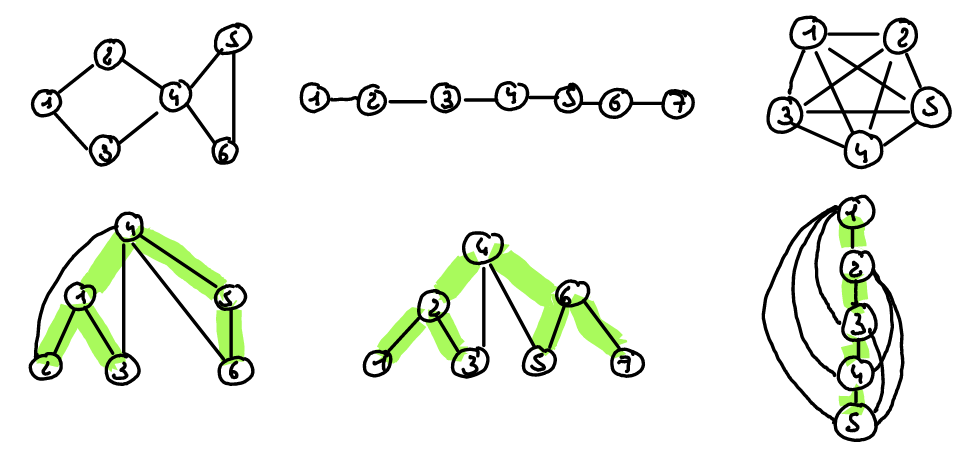
\includegraphics[width=\textwidth]{figures/treedepth-example.png}
    \caption{Examples of treedepth. (a) A graph with treedepth 3. (b) A path of size $n$ has treedepth $\lceil\log_2(n)\rceil$. (c) A clique of size $n$ has treedepth $n$. For each example, the graph is shown at the top, and the elimination forest is depicted in green at the bottom.}
    \label{fig:treedepth-example}
\end{figure}

\medskip

It is quite intuitive why $\pw \lp \td$. Indeed, given a treedepth decomposition of a graph $G$, we can create a bag for every branch of the treedepth decomposition. You can convince yourself that this forms a path decomposition of the graph, and we have $\pw(G) \leq \td(G)$. A pictorial intuition of this transformation is provided \reffigure{fig:treedepth-to-pathwidth}.

\begin{figure}
    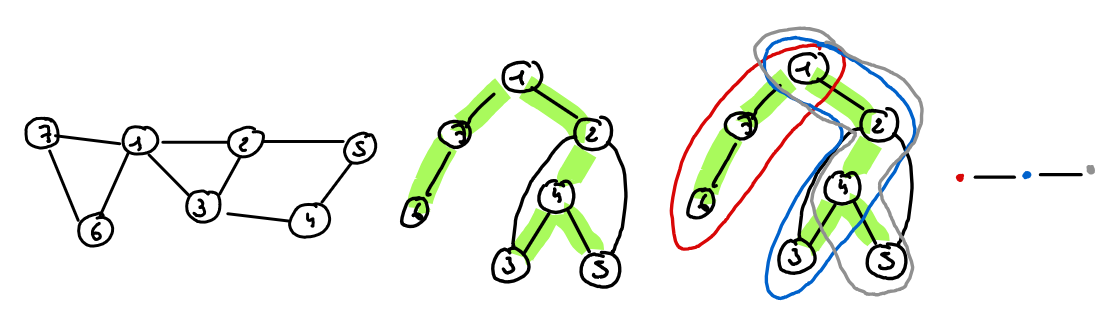
\includegraphics[width=\textwidth]{figures/treedepth-to-pathwidth.png}
    \caption{How to transform an elimination forest into a path decomposition. (a) A graph $G$. (b) An elimination forest of $G$. (c) Bags of a path decomposition of $G$ which follow the elimination forest. (d) The path decomposition of these bags. We can see that the depth of the elimination forest is the same as the width of the obtained path decomposition.}
    \label{fig:treedepth-to-pathwidth}
\end{figure}

\subsubsection*{$\pazocal{F} + kv$ graphs}

Let $\pazocal{F}$ be a class of graphs and $G$ a graph. We say that $G$ is a $\pazocal{F} + kv$ graph if there exists $X \subseteq V(G)$ such that $|X| \leq k$ and $G - X \in \pazocal{F}$. The subset $X$ is called a \textit{hub} and $k$ can be used as a parameter. In this report we will use some of these parameters:

\begin{itemize}
    \item Let $\pazocal{F}$ be \prob{IndependentSet}, the class of all graphs without edges. Then $X$ is a \textit{vertex cover hub} of size $k$, and the parameter is denoted $\vc(G) = k$.
    \item Let $\pazocal{F}$ be \prob{Bipartite}, the class of all graphs without odd cycles. Then $X$ is a \textit{odd cycle transversal hub} of size $k$, and the parameter is denoted $\oct(G) = k$.
    \item Let $\pazocal{F}$ be \prob{Forest}, the class of all graphs without cycles. Then $X$ is a \textit{feedback vertex set hub} of size $k$, and the parameter is denoted $\fvs(G) = k$.
    \item Let $\pazocal{F}$ be \prob{LinearForest}, the class of all graphs without cycles and where the maximum degree of a vertex is 2. Then $X$ is a \todo{find a better name} \textit{linear feedback vertex set hub} of size $k$, and the parameter is denoted $\lfvs(G) = k$.
    \item Let $\pazocal{F}$ be \prob{$\sigma$-ConnectedComponent}, the class of all graphs without connected components of size more than $\sigma$. Then $X$ is a \textit{$\sigma$-hub} of size $k$, and the parameter is denoted $\shub(G) = k$.
\end{itemize}

\medskip

Additionally, we will consider a case for $\sigma$-hub: when the number of edges between each component and $X$ is bounded by a constant $\delta$, then we say that $X$ is a \textit{$(\sigma, \delta)$-hub} of size $k$, and the parameter is denoted $\sdhub(G) = k$.

Examples illustrating each of these parameters can be seen \reffigure{fig:fkv-graph-example}.

\begin{figure}
    \centering
    \begin{subfigure}[b]{0.22\textwidth}
        \adjincludegraphics[width=\textwidth,trim={0 0 {.78\width} 0},clip]{figures/fkv-graph-example.png}
        \caption{A vertex cover of size 7.}
    \end{subfigure}
    \hspace{1cm}
    \begin{subfigure}[b]{0.22\textwidth}
        \adjincludegraphics[width=\textwidth,trim={{.22\width} 0 {.56\width} 0},clip]{figures/fkv-graph-example.png}
        \caption{A feedback vertex set of size 6.}
    \end{subfigure}
    \hspace{1cm}
    \begin{subfigure}[b]{0.18\textwidth}
        \adjincludegraphics[width=\textwidth,trim={{.44\width} 0 {.38\width} 0},clip]{figures/fkv-graph-example.png}
        \caption{A linear feedback vertex set of size 5.}
    \end{subfigure}

    \begin{subfigure}[b]{0.18\textwidth}
        \adjincludegraphics[width=\textwidth,trim={{.62\width} 0 {.2\width} 0},clip]{figures/fkv-graph-example.png}
        \caption{An odd cycle transversal of size 8.}
    \end{subfigure}
    \hspace{1cm}
    \begin{subfigure}[b]{0.2\textwidth}
        \adjincludegraphics[width=\textwidth,trim={{.8\width} 0 0 0},clip]{figures/fkv-graph-example.png}
        \caption{A $(4, 3)$-hub of size 9.}
    \end{subfigure}

    

    \caption{Examples of $\F$-modulators, with the $\F$-modulator drawn in red.}
    \label{fig:fkv-graph-example}
\end{figure}

\medskip

Once again, it is quite intuitive why we have $\oct \lp \fvs \lp \lfvs \lp \shub[2] \lp \vc \lp n$. This is due to the fact that these classes of graphs aleady form a hierarchy:
$$\prob{IndependentSet} \subseteq \prob{$2$-ConnectedComponent} \subseteq \prob{LinearForest} \subseteq \prob{Forest} \subseteq \prob{Bipartite}$$

The first inclusion is due to the fact that if $\sigma \leq \mu$, then $\sigma\prob{-ConnectedComponent} \subseteq \mu\prob{-ConnectedComponent}$. Moreover, \prob{IndependentSet} is the same class as \prob{$1$-ConnectedComponent}, since a graph without edges consists of disconnected components with only one vertex each and vice versa.

Now, if $\pazocal{F}_1 \subseteq \pazocal{F}_2$ and $X$ is a hub such that $G - X \in \pazocal{F}_1$, then $X$ is also a hub such that $G - X \in \pazocal{F}_2$. This explains why $\oct \lp \fvs \lp \lfvs \lp \shub[2] \lp \vc$. Following the same logic, a $\sdhub$ is obviously also a $\shub$, which explains why $\shub \lp \sdhub$. Finally $\vc \lp n$ is quite ovious: a vertex cover of a graph cannot have more vertices than the graph itself.

\medskip

We still need to establish that $\td \lp \shub$, $\tw \lp \fvs$ and $\pw \lp \lfvs$.

\medskip

Let $G$ be a graph with a $\shub$ $X$ of size $k$. The treedepth of $X$ is at most $k$ since we can arrange the vertices of $X$ in a linear fashion, forming a trivial treedepth decomposition (see \reffigure{fig:shub-to-treedepth}). Removing $X$ leaves connected components of size at most $\sigma$, each having treedepth at most $\sigma$. Attaching the treedepth decomposition of each component to the last vertex of the treedepth decomposition of $X$ results in a valid treedepth decomposition for $G$ since the connected components have no common edges. This results in a total depth at most $k + \sigma$. Therefore, $\td(G) \leq \shub(G) + \sigma$, leading to $\td \lp \shub$ since $\sigma$ is a constant.

\begin{figure}
    \centering
    \begin{subfigure}[b]{0.33\textwidth}
        \adjincludegraphics[width=\textwidth,trim={0 0 {.45\width} 0},clip]{figures/shub-to-treedepth.png}
        \caption{}
    \end{subfigure}
    \begin{subfigure}[b]{0.27\textwidth}
        \adjincludegraphics[width=\textwidth,trim={{.55\width} 0 0 0},clip]{figures/shub-to-treedepth.png}
        \caption{}
    \end{subfigure}
    
    \caption{How to transform a $\shub$ $X$ into an elimination forest. (a) A $\shub$ of a graph (in red), and the connected components (in blue). (b) The elimination forest of depth $\leq |X| + \sigma$.}
    \label{fig:shub-to-treedepth}
\end{figure}

\medskip

To show that $\tw \lp \fvs$, consider a feedback vertex set (\fvs) hub $X$ of a graph $G$. Removing $X$ from $G$ results in a forest, and the treewidth of a forest is 1. Thus, we can construct a tree decomposition $T$ for this forest, where each bag has size at most 2. Extend $T$ to $G$ by adding $X$ to each bag results in a tree decomposition $T'$ of $G$ where each bag has size at most $|X| + 2$. Therefore $\tw(G) \leq |X| + 1 = \fvs(G) + 1$, demonstrating that $\tw \lp \fvs$.

\medskip

Observing that removing a linear feedback vertex set (\lfvs) hub from a graph $G$ leaves a forest of path and leads to the same conclusion for $\pw \lp \lfvs$.

\subsubsection*{Certificates}

When designing an algorithm parameterized by a specific parameter, it is crucial to assume that an appropriate \textit{certificate} to this parameter is provided with the input. For instance, when developing an algorithm parameterized by treewidth, we expect a tree decomposition to be provided with the input.

Similarly, for pathwidth, a path decomposition serves as the certificate; for treedepth, it is a treedepth decomposition; and for $\pazocal{F} + kv$ graphs, it is a hub $X$ of size at most $k$.

Therefore, to establish a robust hierarchy of parameters, it is essential that given a upper parameter and its corresponding certificate, we can polynomially construct a certificate for the lower parameter. Fortunately, based on the proofs we've discussed thus far, this polynomial construction of certificates follows naturally.

\medskip

A brief note on $\pazocal{F} + kv$ graphs: when a hub is given, it may not necessarily have the smallest possible size. For instance, a vertex cover hub doesn't lead directly to a polynomial-time algorithm for solving the \prob{VertexCover} problem because there might exist a better vertex cover.

\subsection{Bounds under SETH}

Let $\Pi$ be a problem and $\pi$ a parameter. By $\Pi/\pi$, we denote the problem $\Pi$ parameterized by $\pi$.

\begin{observation}
    \label{obs:upper_bound}
    Let $\Pi$ be a problem, and $\pi_1$ and $\pi_2$ two parameters. If $\pi_1 \lp \pi_2$ and there exists an algorithm for $\Pi/\pi_1$ with running time $\O^\star(q^{\pi_1})$ for a constant $q$, then there exists an algorithm for $\Pi/\pi_2$ with running time $\O^\star(q^{\pi_2})$.
\end{observation}

\begin{proof}
    This observation directly follows from our definition of the hierarchy. Suppose you have a certificate for $\pi_2(G)$, then you can polynomially construct a certificate for $\pi_1(G)$ of same size up to a constant $c$. Thus, we can use the algorithm for $\Pi/\pi_1$, which leads to a time complexity $\O^\star(n^{\O(1)} + q^{\pi_2 + c}) = \O^\star(q^{\pi_2})$, as the $\O^\star$ notation removes polynomial factors. 
\end{proof}

For example, suppose you have an algorithm for $\prob{VertexCover}/\fvs$ in $\O^\star(1.9^\fvs)$, since a $\lfvs$-hub is also a $\fvs$-hub, then you can use the same algorithm for $\prob{VertexCover}/\lfvs$, giving you an $\O^\star(1.9^\lfvs)$ time algorithm.

\begin{observation}
    \label{obs:lower_bound}
    Let $\Pi$ be a problem, and $\pi_1$ and $\pi_2$ two parameters. If $\pi_1 \lp \pi_2$ and there exists no algorithm for $\Pi/\pi_2$ with running time $\O^\star(q^{\pi_2})$ for a constant $q$, then there exists no algorithm for $\Pi/\pi_1$ with running time $\O^\star(q^{\pi_1})$.
\end{observation}

\begin{proof}
    This observation is exactly the contraposite of \refobservation{obs:upper_bound}
\end{proof}

\medskip

These two observations will help you to understand the state of the art described \reffigure{fig:state-of-the-art}.

\subsubsection*{State of the art}

\begin{figure}
    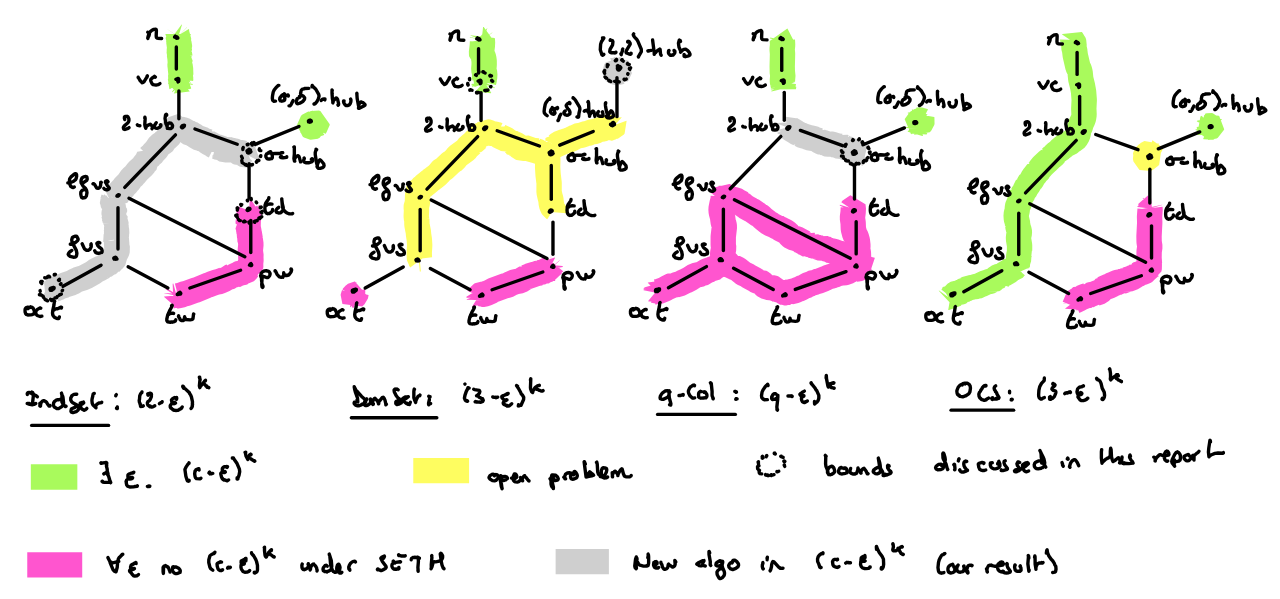
\includegraphics[width=\textwidth]{figures/state-of-the-art.png}
    \caption{Bounds for several \NP-hard problems. For each \NP-hard problem, we consider a constant $c$ and investigate whether there is an algorithm running in time $\O^\star((c-\varepsilon)^k)$ for some parameter $k$ and some $\varepsilon > 0$.}
    \label{fig:state-of-the-art}
\end{figure}

Everything described in this section is illustrated \reffigure{fig:state-of-the-art}.

\medskip

First, note that \prob{VertexCover} and \prob{IndependentSet} are inherently the same problem. Finding an algorithm (or proving that no algorithm exists) for $\prob{VertexCover}/\pi$ for a parameter $\pi$ is equivalent to finding an algorithm (or proving that no algorithm exists) for $\prob{IndependentSet}/\pi$. This is because, for a graph $G$, the size of the maximum independent set and the size of the minimum vertex cover of $G$ sum to $n$, the number of vertices in $G$. Thus, answering the question "is there a \prob{VertexCover} of size $\leq k$?" can be rephrased as "is there no \prob{IndependentSet} of size $\geq n - k + 1$?".

\medskip

\reftheorem{theorem:treewidth-bound} already states the lower bounds parameterized by treewidth for all the problems discussed here. Actually, in this paper, Loshktanov et al. proved the lower bounds under pathwidth \cite{lokshtanov2011known}.

In 2024, Esmer et al. introduces the notion of $\sdhub$ \cite{esmer2024fundamental}. In their paper, they wrote about this parameter: "[$\sdhub$ reached] the arguably most restricted setting in which the lower bounds hold". This message was derived from the following theorems:

\begin{theorem}[\cite{esmer2024fundamental}]
    \label{theorem:sdhub-lowerbounds}
    For every $\varepsilon > 0$ there exist integers $\sigma, \delta \geq 1$ such that if there is an algorithm solving
    \begin{itemize}
        \item $\prob{IndependentSet}/\sdhub$ in time $\O^\star((2 - \varepsilon)^p)$, or
        \item $\prob{OddCycleTransversal}/\sdhub$ in time $\O^\star((3 - \varepsilon)^p)$, or
        \item $q\prob{-Coloring}/\sdhub$ in time $\O^\star((q - \varepsilon)^p)$,
    \end{itemize}
    given with a $\sdhub$ of size at most $p$, then the SETH fails.
\end{theorem}

\begin{theorem}[\cite{esmer2024fundamental}]
    \label{theorem:sdhub-upperbounds}
    For every $\sigma, \delta > 0$, 
    \begin{itemize}
        \item there exists $\varepsilon > 0$ such that every instance of $\prob{IndependentSet}/\sdhub$, can be solved in time $\O^\star((2 - \varepsilon)^p)$,
        \item there exists $\varepsilon > 0$ such that every instance of $\prob{OddCycleTransversal}/\sdhub$ can be solved in time $\O^\star((3 - \varepsilon)^p)$,
        \item there exists $\varepsilon > 0$ such that every instance of $q\prob{-Coloring}/\sdhub$ can be solved in time $\O^\star((q - \varepsilon)^p)$.
    \end{itemize}
    given with a $\sdhub$ of size at most $p$.
\end{theorem}

While \reftheorem{theorem:sdhub-upperbounds} directly provides an algorithm for the three problems. \reftheorem{theorem:sdhub-lowerbounds} is not exactly cited as we want, since $\varepsilon$ is fixed before $\sigma$ and $\delta$. However, \reftheorem{theorem:sdhub-lowerbounds} gives us the following corollary:

\begin{corollary}
    \label{corollary:td-lowerbounds}
    For every $\varepsilon > 0$, if there is an algorithm solving
    \begin{itemize}
        \item $\prob{IndependentSet}/\td$ in time $\O^\star((2 - \varepsilon)^\td)$, or
        \item $\prob{OddCycleTransversal}/\td$ in time $\O^\star((3 - \varepsilon)^\td)$, or
        \item $q\prob{-Coloring}/\td$ in time $\O^\star((q - \varepsilon)^\td)$,
    \end{itemize}
    then the SETH fails.
\end{corollary}

\begin{proof}
    Let's prove this for $\prob{IndependentSet}$; the proof for $\prob{OddCycleTransversal}$ and \prob{$q$-Coloring} is analogous.

    Suppose there exists an $\varepsilon$ such that there is an algorithm solving $\prob{IndependentSet}/\td$ in time $\O^\star((2 - \varepsilon)^\td)$. Take $\sigma$ and $\delta$ given for this $\varepsilon$ by \reftheorem{theorem:sdhub-lowerbounds}. Given a $\sdhub$ of size $p$, we can transform it into a treedepth decomposition of depth $p + \sigma$ as described in the previous section (see \reffigure{fig:shub-to-treedepth}). By applying the algorithm for $\prob{IndependentSet}/\td$, we get a time complexity of $\O^\star((2 - \varepsilon)^{p + \sigma}) = \O^\star((2 - \varepsilon)^p)$. By \reftheorem{theorem:sdhub-lowerbounds}, SETH fails.
\end{proof}

Note that Esmer et al. did not establish the same bounds for $\prob{DominatingSet}\sdhub$, leaving this as an open problem.

\medskip

$\prob{IndependentSet}/\vc$ is a well studied algorithm and can run in ??\todo{find a bound and a citation here}.

\medskip

\prob{DominatingSet} is already \NP-hard on bipartite graphs. Thus, finding an algorithm for $\prob{DominatingSet}/\oct$  with running time $\O^\star((3-\varepsilon)^\oct)$ is highly improbable unless $\P = \NP$, which is a stronger conjecture than SETH. Moreover, an algorithm for $\prob{DominatingSet}/\vc$ can run in $\O^\star(2^\vc)$; we will discuss this \refsec{section:domset-vc}.

\medskip

A few years after the work by Loshkatnov et al., Jaffke and Jansen extended it and proved a lower bound for $q\prob{-Coloring}/\lfvs$ \cite{jaffke2017fine}. They also proposed an algorithm running in time $\O^\star((q - 1.11)^\vc)$ for $q\prob{-Coloring}/\vc$.

\medskip

Finally, an algorithm for $\prob{OddCycleTransversal}/\oct$ was proposed by Narayanaswamy et al. \cite{narayanaswamy2012lp}, who developed an algorithm based on a branching guided by linear programming that runs in time $\O^\star(2.68^\oct)$. This was later improved by Lokshtanov et al. \cite{lokshtanov2012subexponential} to $\O^\star(2.32^\oct)$. 

\subsubsection*{Our result}

\todo{there are probably too many sections}

The goal of this internship was to find new upper and lower bounds under SETH. While the main focus was initially on \prob{DominatinSet}, we didn't achieved new interesting results for this problem. However, we developed an algorithm for $\prob{DominatingSet}/\sdhub[2, 2]$ running in time $\O^\star(2^p)$, given a $\sdhub[2,2]$ of size $p$. This algorithm solves a somewhat useless problem but demonstrates our methodology. More details on this algorithm are discussed \refsec{section:domset-22hub}.

\medskip

We found interesting results for $\prob{IndependentSet}/\oct$ and proposed an algorithm with a running time $\O^\star((\sqrt{2.32})^\oct)$ (see \refsec{section:indset-oct}). While the bound for $\prob{IndependentSet}/\td$ was already clear by \refcorollary{corollary:td-lowerbounds}, we found an alternative proof showing this lower bound, which is presented \refsec{section:indset-td}. Additionally, we completed the hierarchy bounds for \prob{IndependentSet} by showing that for every $\sigma$, there exists an $\varepsilon$ such that $\prob{IndependentSet}/\shub$ can be solved in $\O^\star((2- \varepsilon)^p)$ given a $\shub$ of size $p$. This algorithm is detailed \refsec{section:indset-shub}.

\medskip

To further complete the hierarchy bounds for \prob{$q$-Coloring}, we extended the work of Esmer et al. to show that for every $\sigma$, there exists an $\varepsilon$ for which there is an algorithm solving \prob{$q$-Coloring} in time $\O^\star((q-\varepsilon)^p)$ given a $\shub$ of size $p$. This algorithm is detailed \refsec{section:qcol-shub}.